\documentclass[12pt]{article}

\usepackage[affil-it]{authblk}
\usepackage[shortlabels]{enumitem}
\usepackage[utf8]{inputenc}
\usepackage{algorithm, algorithmicx, algpseudocode}
\usepackage{amsfonts, amsthm, amsmath, amssymb}
\usepackage{color}
\usepackage{cancel, textcomp}
\usepackage{enumerate}
\usepackage[mathscr]{euscript}
\usepackage{fancyhdr, fancyvrb}
\usepackage{fullpage}
\usepackage[left=0.5in,right=0.5in,headsep=0.5in,headheight=0.5in]{geometry}
\usepackage{graphicx}
\usepackage{hyperref}
\usepackage{latexsym}
\usepackage{mathtools}
\usepackage{minted}
\usepackage{times}
\usepackage{xcolor}
\usepackage{physics}
\usepackage{tikz-cd}
\usepackage[warnunknown, fasterrors, mathletters]{ucs}
\usepackage[nointegrals]{wasysym}

\newcommand{\hw}[2]{
    \noindent
    \begin{center}
        \framebox{
            \vbox{
                \hbox to 7in { {\bf MATH 470: Communications and Cryptography } \hfill  }
                \vspace{2mm}
                \hbox to 7in { {\Large \hfill Homework #1\hfill} }
                \vspace{2mm}
                \hbox to 7in { {\it Due date: #2 \hfill Name: Huy Lai } }
            }
        }
    \end{center}
    \vspace*{4mm}
}

\newcounter{prob}
\setcounter{prob}{0}
\newcounter{subprob}
\setcounter{subprob}{0}

\newcommand{\problem}{\setcounter{subprob}{0}\stepcounter{prob}{\noindent\textbf{Problem \theprob.}}\ }
\newcommand{\subproblem}{\stepcounter{subprob}{\noindent\textbf{Subproblem \thesubprob.}}\ }
\newcommand{\solution}{\noindent\textbf{Solution:}\newline}

\newcommand{\babc}{\begin{enumerate}[a)]}
\newcommand{\eabc}{\end{enumerate}}

\everymath{\displaystyle}

\setlength{\parskip}{.1in}
\setlength{\headheight}{15pt}
\setlength{\topmargin}{0pt}

\fancyhf{}
\pagestyle{fancy}
\lhead{MATH 470: Communications and Cryptography}
\rhead{Texas A\&M University}
\cfoot{\thepage}


\begin{document}
\hw{6}{12 October 2023}
\thispagestyle{empty}
\problem Let $N=pq$ be the product of two distinct primes. Let $e,d$ be integers such that $ed\equiv1\mod{\phi(N)}$. Prove that for every integer $m$, we have $m^{ed}\equiv m\mod{N}$. (note: If $\gcd(m,N)=1$, then this follows from the Proposition from class that $m^{\phi(N)}\equiv 1\mod{N}$. The purpose of this problem is to handle the other cases, thus proving that RSA decryption always returns the original message.)

\solution The proof is as follows
\begin{proof}
    We can use the Chinese Remainder Theorem to show that the two congruences
    \[m^{ed}\equiv m\mod{p}\quad\text{ and }\quad m^{ed}\equiv m\mod{q}\]
    hold.\\
    We can use the fact that $\gcd(p,q)=1$ and the Chinese Remainder Theorem to show that $m^{ed}\equiv m\mod{N}$.

    \noindent
    By proposition, $ed\equiv1\mod{\phi(N)}\rightarrow\phi(N)\mid(ed-1)$\\
    By definition of divisibility, $\exists k\in\mathbb{Z}$ such that $k\cdot\phi(N)=ed-1\rightarrow ed=k\cdot\phi(N)+1$

    \noindent
    If $m\equiv0\mod{p}$, then certainly $m^{ed}\equiv m\mod{p}$.\\
    If $m\not\equiv0\mod{p}$, then by Fermat's Little Theorem, $m^{p-1}\equiv 1\mod{p}$.\\
    From this we get the following:
    \[m^{ed}\equiv m^{k\cdot\phi(N)+1}\equiv m(m^{p-1})^{k(q-1)}\equiv m\cdot 1^{k(q-1)}\equiv m\mod{p}\]
    Therefore, $m^{ed}\equiv m\mod{p}$ holds for all integers $m$.\\
    Replacing $p$ with $q$ in the previous argument shows that $m^{ed}\equiv m\mod{q}$ holds for all integers $m$.
\end{proof}

\newpage
\problem For each part, use the data provided to find values of $a$ and $b$ satisfying $a^2\equiv b^2\mod{N}$, and then compute $\gcd(N,a-b)$ in order to find a nontrivial factor of $N$, as we did in Examples 3.37 and 3.38. $N = 2525891$

\solution
First we try
\begin{flalign*}
    1591^2\cdot 3182^2          & \equiv(2\cdot5\cdot7^2\cdot11)(2^3\cdot5\cdot7^2\cdot11)\mod{N} & \\
                                & =(2^2\cdot5\cdot7^2\cdot11)^2                                   & \\
                                & =10780^2                                                        & \\
    \gcd(N,1591\cdot3182-10780) & = 2525891                                                       &
\end{flalign*}

\noindent
Next we try
\begin{flalign*}
    1591^2\cdot 4773^2          & \equiv(2\cdot5\cdot7^2\cdot11)(2\cdot3^2\cdot5\cdot7^2\cdot11)\mod{N} & \\
                                & =(2\cdot3\cdot5\cdot7^2\cdot11)^2                                     & \\
                                & =16170^2                                                              & \\
    \gcd(N,1591\cdot4773-16170) & = 2525891                                                             &
\end{flalign*}

\noindent
Next we try
\begin{flalign*}
    3182^2 \cdot 4473^2               & \equiv (2^3\cdot5\cdot7^2\cdot11)(2\cdot3^2\cdot5\cdot7^2\cdot11) & \\
                                      & \equiv (2^2\cdot3\cdot5\cdot7^2\cdot11)^2                         & \\
                                      & \equiv 32340^2 \mod{N}                                              \\
    \gcd(2525891,3182\cdot4473-32340) & = 2525891                                                         &
\end{flalign*}

\noindent
Finally we try
\begin{flalign*}
    1591^2\cdot 5275^2\cdot 5401^2          & \equiv(2\cdot5\cdot7^2\cdot11)(2^3\cdot3^6\cdot7)(2^4\cdot3^2\cdot5^3\cdot7\cdot11)\mod{N} & \\
                                            & =(2^4\cdot3^4\cdot5^2\cdot7^2\cdot11)^2                                                    & \\
                                            & =17463600^2                                                                                & \\
    \gcd(N,1591\cdot5275\cdot5401-17463600) & = 1637                                                                                     &
\end{flalign*}

\newpage
\problem Let $L(N)=e^{\sqrt{\ln{N}\ln{\ln{N}}}}$ as ususal. Suppose that a computer does one billion operations per second.
\begin{enumerate}
    \item How many seconds does it take to perform $L(2^{100})$ operations?
    \item How many hours does it take to perform $L(2^{250})$ operations?
    \item How many days does it take to perform $L(2^{350})$ operations?
    \item How many years does it take to perform $L(2^{500})$ operations?
    \item How many years does it take to perform $L(2^{750})$ operations?
    \item How many years does it take to perform $L(2^{1000})$ operations?
    \item How many years does it take to perform $L(2^{2000})$ operations?
\end{enumerate}

\solution The length of the operations is as follows
\begin{enumerate}
    \item $2.780\cdot10^{-2}$ sec
    \item $2.657\cdot10^{0}$ hr
    \item $8.224\cdot10^{1}$ days
    \item $1.129\cdot10^{3}$ years
    \item $1.833\cdot10^{8}$ years
    \item $5.548\cdot10^{12}$ years
    \item $9.846\cdot10^{35}$ years
\end{enumerate}

\newpage
\problem Implement Pollard's $p-1$ algorithm on a computer to factor $N$:
\[N=340510176929609558738506407941198102081020749940944635553628097992090306553579338501\]

\solution
The algorithm is as follows
\inputminted{python3}{pollard.py}

\begin{figure}[!ht]
    \centering
    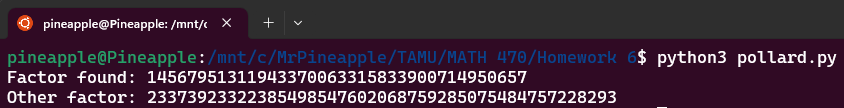
\includegraphics[width=\textwidth]{q4.png}
    \caption{Output}
\end{figure}

\newpage
\problem Let $p$ be an odd prime and let $g$ be a primitive root modulo $p$. Then any number $a$ is equal to some power of $g\mod{p}$, say $a\equiv g^k\mod{p}$. Prove that $a$ has a square root modulo $p$ if and only if $k$ is even.

\solution
We first prove that if $k$ is even, then $a$ has a square root modulo $p$.
\begin{proof}
    Assume $k$ is an even integer such that $k=2j$. Then
    \[a\equiv g^k\equiv g^{2j}\equiv (g^j)^2\mod{p}\]
    $\therefore$ $a$ has a square root modulo $p$
\end{proof}

\noindent
Next we prove that if $a$ has a square root modulo $p$ then $k$ is even.
\begin{proof}
    Assume $a$ is a square such that $a\equiv b^2\mod{p}$\\
    Since $g$ is a primitive root, $b\equiv g^i\mod{p}$ for some integer $i$. Then
    \[g^k\equiv a\equiv b^2\equiv (g^i)^2\equiv g^{2i}\mod{p}\]
    Multiplying both sides by the inverse of $g^{2i}$ gives us:
    \[g^{k-2i}\equiv 1\mod{p}\]
    The fact that $g$ is a primitive root implies that $p-1\mid(k-2i)$.\\
    We know that $p-1$ is even. Therefore $2\mid(p-1)$\\
    By proposition, if $2\mid(p-1)$ and $p-1\mid(k-2i)$, then $2\mid(k-2i)$.\\
    Additionally, by proposition, $2\mid(k-2i)\rightarrow 2\mid k$ and $2\mid 2i$.\\
    Therefore, $k$ is even.
\end{proof}

\newpage
\problem Let $k$ be a positive integer. What is the number of square roots of $1\mod{2^k}$? In order words, determine the number integer $x$ with $0\leq x\leq 2^k-1$ that satisfy $x^2\equiv 1\mod{2^k}$.

\solution
When $k=1$, there is only one solution: $x=1$\\
When $k=2$, there are two solutions: $x=1,x=3$

\noindent
We will now handle when $k\geq3$\\
Let $x$ be am integer such that $x^2\equiv1\mod{2^k}$.\\
Rearranging gives us $(x-1)(x+1)\equiv0\mod{2^k}$.

\noindent
Since $x\equiv1\mod{2}$, $x\pm1\equiv0\mod{2}$.\\
Because of this $\gcd(x-1,x+1)=2$, which implies that one of $x\pm1\equiv2\mod{4}$.

\noindent
Since $2^k\mid(x-1)(x+1)$, one of $x\pm1$ is divisible by $2^{k-1}$, which means $x\pm1\equiv0$ or $2^{k-1}\mod{2^k}$.\\
If $x\pm1\equiv0\mod{2^k}$, then we get two solutions $x\equiv1\mod{2^k}$ and $x\equiv-1\mod{2^k}$\\
If $x\pm1\equiv2^{k-1}\mod{2^k}$, then we get two more solutions $x\equiv2^{k-1}-1\mod{2^k}$ and $x\equiv2^{k-1}+1\mod{2^k}$

\noindent
Therefore, when $k\geq3$, there are four solutions: $x=1,x=2^{k-1}-1,x^{k-1}+1,x=2^k-1$

\newpage
\problem Let $p$ be an odd prime and let $b$ be an integer not divisible by $p$. Prove that for every positive integer $e$, the congruence $X^2\equiv b\mod{p^e}$ has either $0$ or $2$ solutions in $\mathbb{Z}/p^e\mathbb{Z}$.

\solution
The proof is as follows
\begin{proof}
    Base Case: $e=1$\\
    $X^2\equiv b\mod{p^1}$ has 0 or 2 solutions is proven by Homework 3 Question 4.

    \noindent
    If $X^2\equiv b\mod{p^1}$ has a solution, then $X^2\equiv b\mod{p^2}$ also has a solution is proven by is proven by Homework 4 Question 5.

    \noindent
    Inductive Hypothesis\\
    Assume that if $X^2\equiv b\mod{p^{e}}$ has a solution in $\mathbb{Z}/p^{e+1}\mathbb{Z}$ then $X^2\equiv b\mod{p^{e+1}}$ also has a solution $\forall e\geq 1$.\\
    Additionally, assume that $X^2\equiv b\mod{p^{e}}$ has two unique solutions.

    \noindent
    Inductive Step\\
    Without loss of generality, let $\alpha$ be a solution to the congruence $X^2\equiv b\mod{p^e}$.\\
    By the inductive hypothesis, we also have a solution $\beta$ that solve the congruence $X^2\equiv b\mod{p^{e+1}}$.\\
    From homework 4 question 5, we know we can generate the solution $\beta$ from $\alpha$ by adding a multiple of $p^e$.

    \noindent
    A similar logic can be applied to the other solution to the congruence $X^2\equiv b\mod{p^e}$.
\end{proof}
\end{document}
